\subsection*{Exeecise 7.1 : An electromagnetic relay}
We consider the state model given in exemple 3.2:
\begin{align*}
\dot{x}_1 &= x_2 \\
\dot{x}_2 &= \frac{k}{m}(z_0-x_1) - \frac{\alpha \beta}{2m} \left( \frac{x_3}{1+\beta x_1} \right)^2 \\
\dot{x}_3 &= \frac{\beta x_2 x_3}{1+\beta x_1} - \frac{R}{\alpha} (1+\beta x_1)x_3 + \frac{1+\beta x_1}{\alpha} u
\end{align*}
The equilibrium point is given by:
\begin{align*}
0 &=  \bar{x}_2 \\
0 &= \frac{k}{m}(z_0-\bar{x}_1) - \frac{\alpha \beta}{2m} \left( \frac{\bar{x}_3}{1+\beta \bar{x}_1} \right)^2 \\
0 &= \frac{\beta \bar{x}_2 \bar{x}_3}{1+\beta \bar{x}_1} - \frac{R}{\alpha} (1+\beta \bar{x}_1)\bar{x}_3 + \frac{1+\beta \bar{x}_1}{\alpha} \bar{u}
\end{align*}
By replacing $\bar{x}_2$ by its value in the third equation we find: 
\begin{align*}
0 &=  \bar{x}_2 \\
0 &= \frac{k}{m}(z_0-\bar{x}_1) - \frac{\alpha \beta}{2m} \left( \frac{\bar{x}_3}{1+\beta \bar{x}_1} \right)^2 \\
0 &=  -\frac{R}{\alpha} (1+\beta \bar{x}_1)\bar{x}_3 + \frac{1+\beta \bar{x}_1}{\alpha} \bar{u}
\end{align*}
With the third equation we obtain : $\bar{x}_3 = \frac{\bar{u}}{R}$\\
We replace $\bar{x}_3$ by its value in the second equation:
\begin{align*}
0 &= \frac{k}{m}(z_0-\bar{x}_1) - \frac{\alpha \beta}{2m} \left( \frac{\frac{\bar{u}}{R}}{1+\beta \bar{x}_1} \right)^2 \\
&\Rightarrow  \frac{k}{m}(z_0-\bar{x}_1) = \frac{\alpha \beta}{2m} \left( \frac{\frac{\bar{u}}{R}}{1+\beta \bar{x}_1} \right)^2 \\
&\Rightarrow  2k(z_0-\bar{x}_1) (1+\beta \bar{x}_1)^2 = \alpha \beta \left( \frac{\bar{u}}{R} \right)^2  \\
\end{align*}
We can analyse this equation graphically (see figure \ref{Graphe7_1}). But we know that the feasible points verify: $0 \le \bar{x}_1 \le z_0$. 
We use the function $\bar{u}^2 = \frac{2R^2}{\alpha \beta} (z_0-x)(1+\beta x)^2 $.
\begin{itemize}
\item We find the roots $x = z_0$ and $x = \frac{-1}{\beta} $
\item We define the intercept: $B = \frac{2R^2}{\alpha \beta} z_0 $
\item We find the extrema of the function: \begin{align*}
\frac{d\left[ (z_0 - x) (1+ \beta x)^2 \right]}{dx} &= 0 \\
\Rightarrow  2 \beta (z_0 - x) (1+ \beta x) - (1+ \beta x)^2 &= 0 \\
\Rightarrow   (1+ \beta x)     \left( 2 \beta (z_0 - x)- (1+ \beta x) \right) &= 0 \\
\end{align*}
We obtain a local minimum for $x = \frac{-1}{\beta}$ and a local maximum for $x = \frac{2\beta z_0 -1}{3 \beta} $ (Note that the function is in fact unbounded over $\mathbb{R}$).
We define $A$ the value of the local maximum.
\end{itemize}

We know that $\frac{-1}{\beta}$ is always negative. However the maximum can be positive or negative according to the value : $2\beta z_0 -1 $. \\
 We analyse now the two cases: 
\begin{itemize}
\item If $2\beta z_0 > 1$, we have: 
 \begin{itemize}
\item An equilibrium for $0 \le \bar{u}^2 \le B $ 
\item Two equilibria for $B \le \bar{u}^2 \le A  $
\item An equilibrium for $\bar{u}^2 = A  $
\item No equilibrium for $ \bar{u}^2 \ge A  $
\end{itemize}
\item If $2\beta z_0 \le 1$, we have: 
\begin{itemize}
\item According to the value of $\bar{u}$, there is one or zero equilibrium. 
\end{itemize}
\end{itemize}

\begin{figure}
\centering
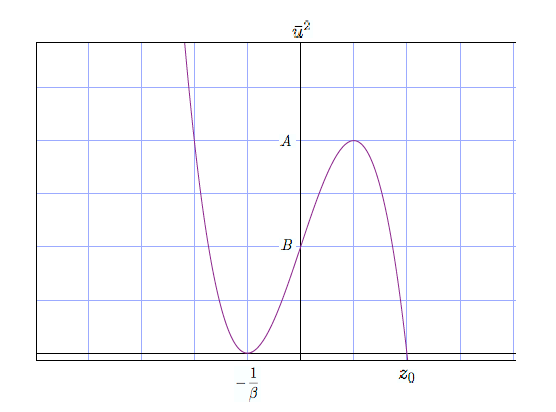
\includegraphics[scale=0.5]{Graphe7_1}
\caption{Graph of $\frac{2R^2}{\alpha \beta} (z_0-x)(1+\beta x)^2 $}.
\label{Graphe7_1}
\end{figure}

\subsection*{Exercise 7.2 : DC Generator}
We consider a DC generator. The equations are given in section 3.9. We also use the fact that the viscous friction is linear: 
\begin{align*}
L_s \dot{x_1} &= -R_s x_1 + u_1 \\
L_r \dot{x_2} &= -\left( R_L + R_r \right) x_2 - K_e x_3x_1 \\
J \dot{x}_3 &= -h(x_3) + K_m x_1 x_2 + u_2   
\end{align*}
The equilibrium point is given by:
\begin{align*}
0 &= -R_s \bar{x}_1 + \bar{u}_1 \\
0 &= -\left( R_r + R_L \right) \bar{x}_2 - K_e \bar{x}_3 \bar{x}_1 \\
0 &= -h(\bar{x}_3) + K_m \bar{x}_1 \bar{x}_2 + \bar{u}_2   
\end{align*}
We find $ \bar{x}_1 = \frac{\bar{u}_1}{R_s}$ and replace it by its value in the other equations: 
\begin{align*}
\bar{x}_1 &= \frac{\bar{u}_1}{R_s} \\
0 &= -\left( R_r + R_L \right) \bar{x}_2 - K_e \bar{x}_3 \frac{\bar{u}_1}{R_s}  \\
0 &= -h(\bar{x}_3) + K_m  \bar{x}_2 \frac{\bar{u}_1}{R_s}  + \bar{u}_2   
\end{align*}
We put the value of $\bar{x_3} = K_m  \bar{x}_2 \frac{\bar{u}_1}{R_s h}  + \frac{\bar{u}_2}{h}  $ in the second equation to find $\bar{x}_2$:
\begin{align*}
0 &= -\left( R_r + R_L \right) \bar{x}_2 - K_e \left( K_m  \bar{x}_2 \frac{\bar{u}_1}{R_s h}  + \frac{\bar{u}_2}{h}  \right)  \frac{\bar{u}_1}{R_s}  \\
0 &= - R_s^2 h\left( R_r + R_L \right) \bar{x}_2 - K_e \left( K_m  \bar{x}_2 \bar{u}_1  + R_s \bar{u}_2  \right)  \bar{u}_1  \\
\left( R_s^2 h\left( R_r + R_L \right) + K_e  K_m \bar{u}_1^2  \right) \bar{x}_2 &= - K_e R_s \bar{u}_1 \bar{u}_2 \\
\bar{x}_2 &= \frac{- K_e R_s \bar{u}_1 \bar{u}_2}{R_s^2 h\left( R_r + R_L \right) + K_e  K_m \bar{u}_1^2}
\end{align*}
The value $\bar{x_3}$ is given by: \\
$$\bar{x_3} = K_m  \left(  \frac{- K_e R_s \bar{u}_1 \bar{u}_2}{R_s^2 h\left( R_r + R_L \right) + K_e  K_m \bar{u}_1^2} \right) \frac{\bar{u}_1}{R_s h}  + \frac{\bar{u}_2}{h}  $$
Lastly we obtain: 
\begin{align*}
\bar{x}_1 &= \frac{\bar{u}_1}{R_s} \\
\bar{x}_2 &= \frac{- K_e R_s \bar{u}_1 \bar{u}_2}{R_s^2 h\left( R_r + R_L \right) + K_e  K_m \bar{u}_1^2} \\
\bar{x_3} &= \frac{K_m}{h}  \left(  \frac{- K_e R_s \bar{u}_1 \bar{u}_2}{R_s^2 h\left( R_r + R_L \right) + K_e  K_m \bar{u}_1^2} \right) \frac{\bar{u}_1}{R_s}  + \frac{\bar{u}_2}{h}
\end{align*}

\subsection*{Exercise 7.3 : Grinding Mill}
\underline{1. Compartments
system graph}

{\centering
\includegraphics[scale=0.7]{Graphe7_3_1}
%\caption{}
\label{Graphe7_3_1}

}

\underline{2. Equilibria} \\
Equilibria satisfy the following relationships:
\begin{align*}
\gamma_1\bar{x}_1 &= \bar{u} \\
\gamma_2\bar{x}_2 &= \frac{\alpha }{1-\alpha }\bar{u} \\
(1-\alpha )\phi (\bar{x}_3) &= \bar{u}
\end{align*}
The last equality can be analyzed graphically (see figure below). We observe that, depending on the value of $\bar{u}\geq 0$, there is no, one or two equilibria. The figure shows the case with two equilibria.

{\centering
\includegraphics[scale=0.3]{Graphe7_3_2}
%\caption{}
\label{Graphe7_3_2}

}

\underline{3. Invariant} \\
To show that the region is invariant, it is sufficient to show that for a state on the border, the vector field describing the variation of the state points inwards. \\ \\
If we consider a section of the invariant region in the plan $(x_1,x_3)$ as shown in the next figure (green shaded area) two situations should be considered :\\ \\
\indent a) We are on the border $\gamma_1x_1 = \bar{u}$. In this case, the vector points downwards. Indeed, $$\dot{x}_1=-\bar{u}+(1-\alpha )\phi (x_3)\leq 0.$$
\indent b) We are now on the border $\gamma_1x_1 = (1-\alpha )\phi (x_3)$. In this case, the vector points to the right. Indeed, we have $\dot{x}_1 = 0$ and 
\begin{align*}
\dot{x}_3 &= \gamma_2x_2 - \phi (x_3) + \bar{u} \\
&= (\gamma_2x_2 - \alpha\phi (x_3)) + (\bar{u}-(1-\alpha)\phi (x_3)) \geq 0, 
\end{align*}
because each term in this expression is positive for all $(x_1,x_2,x_3)$ in the invariant region. \\
We only need to apply the same reasoning on a section of the plane $(x_2,x_3)$ to end the demonstration. 

{\centering
\includegraphics[scale=0.3]{Graphe7_3_3}
%\caption{}
\label{Graphe7_3_3}

}

\subsection*{Exercise 7.5 : Mechanical system}
\underline{1. State model} \\ \\
Let $x_1 = \theta $, $x_2 = \dot{\theta }$ the system is \\
\indent$ \dot{x}_1 = x_2$ \\
\indent $\dot{x}_2 = -r\sin (x_1)-cx_2 $ \\ \\
\underline{2. Equilibria} \\ \\
\indent$ \theta = k\pi \ \; \forall k\in \mathbb{Z} $\\ \\
\underline{3. Bounded invariant} \\ \\
Let's suppose $c^2 \geq 4r$, the following region is invariant \\
\indent$\mathcal{D} = \{ (x_1,x_2)\ \vert \ 0\leq x_1\leq \pi /2,-\frac{2r}{c}x_1\leq x_2\leq 0\}$